%*-------------------------------------------------------------------------*
%*                 Copyright 2013 Core Physics, Inc.                       *
%*  Under terms of the contract to support CASL, there is a non-exclusive  *
%*  license for use of this work by or on behalf of the U.S. Government.   *
%*-------------------------------------------------------------------------*
%
% @version CVS $Id: verain.tex,v 1.24 2013/11/19 17:28:04 scott Exp $
%
\documentclass{report}
%
%  various packages that you may wish to activate for usage
\usepackage{graphics}
\usepackage{epsfig}
\usepackage{fancyheadings}
\usepackage{amssymb,amsmath}

\numberwithin{equation}{section}

\usepackage[pdftex,
  pdftitle={VERA Common Input},
  pdfauthor={www.casl.gov},
  pdfsubject={ },
  bookmarks, bookmarksopen, bookmarksnumbered,
  pdfstartview={FitH},
  colorlinks,linkcolor={blue},citecolor={blue},
  urlcolor={red}]{hyperref}

\DeclareGraphicsExtensions{.eps}
\DeclareGraphicsRule{.eps}{eps}{}{}

%  standard margins are 1.875in for 10pt document
%  this changes them to 1.25 inch
\addtolength{\oddsidemargin}{-0.525in}
\addtolength{\evensidemargin}{-0.525in}
\addtolength{\textwidth}{1.05in}

\setlength{\parindent}{0in}  % do not indent paragraphs, double space between
\addtolength{\parskip}{1.0\baselineskip}

%% card list - See pg. 75 in book
\newenvironment{cardlist}
 {\begin{list}{}
  {\setlength{\labelwidth}{2.0cm}
   \setlength{\leftmargin}{2.5cm}   % was 2
   \setlength{\labelsep}{0.25cm}    % was 0.5
   \setlength{\rightmargin}{2.0cm}
   \setlength{\topsep}{-0.2cm}
%  \setlength{\parsep}{0.5ex plus0.2ex minus0.5ex}
   \setlength{\itemsep}{0ex plus0.2ex} }}
{\end{list}}

%  Define page headers and footers
\pagestyle{fancy}
\newcommand{\tstamp}{\today}
\renewcommand{\chaptermark}[1]{\markboth{#1}{}}
\renewcommand{\sectionmark}[1]{\markright{#1}}
\lhead[\fancyplain{}{\thepage}]         {\fancyplain{}{\rightmark}}
\chead[\fancyplain{}{}]                 {\fancyplain{}{}}
\rhead[\fancyplain{}{\rightmark}]       {\fancyplain{VERA Common Input}{VERA Common Input}}
\lfoot[\fancyplain{}{}]                 {\fancyplain{}{}}
\cfoot[\fancyplain{\thepage}{}]         {\fancyplain{\thepage}{\thepage}}
\rfoot[\fancyplain{\tstamp} {\tstamp}]  {\fancyplain{}{}}

\begin{document}
%*-------------------------------------------------------------------------*
%*                 Copyright 2013 Core Physics, Inc.                       *
%*  Under terms of the contract to support CASL, there is a non-exclusive  *
%*  license for use of this work by or on behalf of the U.S. Government.   *
%*-------------------------------------------------------------------------*
%
% @version CVS $Id: titlepage.tex,v 1.4 2013/11/19 17:28:04 scott Exp $
%
% Title page
%

\begin{titlepage}
    \centering
    \vfill
    {\bfseries\LARGE
        VERA Common Input}
        \vskip4cm
    {\Large
        Consortium for Advanced Simulation of LWRs (CASL) \\
        www.casl.gov \\
        \vskip2cm
%%      \today
        November 2013 \\
        RSICC Release \\
    }
    \vfill
    \vfill
    
\includegraphics[width=6cm]{figs/casl_sm.jpg}
    \vfill
\end{titlepage}


%%%%%%%%%%%%%%%%%%%%%%%%%%%%%%%%%%%%%%%%%
\tableofcontents

% \listoffigures
%%%%%%%%%%%%%%%%%%%%%%%%%%%%%%%%%%%%%%%%%

\chapter{Introduction}

\section{Introduction to CASL}
The Consortium for Advanced Simulation of Light Water Reactors (CASL) is the first
DOE Energy Innovation Hub established in July 2010, for the purpose of providing
advanced modeling and simulation (M\&S) solutions for commercial nuclear reactors.

CASL’s vision is to predict, with confidence, the performance of nuclear reactors
through comprehensive, science-based modeling and simulation technology that is
deployed and applied broadly throughout the nuclear energy industry to enhance safety,
reliability, and economics.

CASL’s mission is to provide coupled, higher-fidelity, usable modeling and simulation
capabilities needed to address light water reactor operational and safety performance-defining phenomena.

CASL’s foundational technology products include CASL solutions and CASL ModSim Technologies.
CASL’s ModSim technology, the Virtual Environment for Reactor Applications (VERA), provides
higher-fidelity results than the current industry approach by incorporating coupled physics
and science-based models, state-of-the-art numerical methods, modern computational science,
integrated uncertainty quantification (UQ) and validation against data from operating
pressurized water reactors (PWRs), single-effect experiments, and integral tests.

CASL will address, through new insights afforded by its ModSim technology, key nuclear
energy industry challenges to furthering power uprates, higher fuel burnup, and lifetime
extension while providing higher confidence in enhanced nuclear safety and this cleaner energy source.

The CASL Team is a consortium that consists of ten core partners and numerous contributing members.
The CASL organization is led by Oak Ridge National Lab, and CASL’s R\&D is executed
in six technical teams called Focus Areas (FA) and one integrating technical area,
Collaboration and Ideation (C\&I). This ground-breaking partnership provides unparalleled
collective institutional knowledge, nuclear science and engineering talent, computational
science leadership, and a record of LWR design and regulatory accomplishments!

\section{VERA Core Simulator}
One piece of VERA is the VERA Core Simulator.  The core simulator is the specific collection
of multi-physics computer codes used to model and deplete a LWR core over multiple cycles.
Examples of the separate physics codes include cross section models, neutron transport, depletion,
thermal-hydraulics, and fuel performance.

The purpose of the core simulator is to provide data and boundary conditions to model
CASL Challenge Problems such as CIPS, CILC, DNB, and PCI analysis.

One important feature of the core simulator is that a single common input file is used to drive all
of the different physics codes\footnote{The only exception to this is for CFD codes,
which require a CAD drawing to perform any meaningful analysis.}.
One benefit of using a single common input is that users only need to understand and be proficient with one input,
instead of having to understand multiple inputs for multiple physics codes.
Another benefit of using a single common input is that all codes will be working from a single
geometry description and this will reduce errors due to inconsistent models.

This document lives in the VERA GIT repository file ``VERAInExt/verain/docs/verain\_UM.pdf''.  
Please refer to this location for the latest version of the input manual.


%%%%%%%%%%%%%%%%%%%%%%%%%%%%%%%%%%%%%%%%%
\chapter{User Manual}

% fix: add more about input, parsing rules, white space, comments, etc
% fix: add description of units.  Most units are CGS, but there are exceptions.  See Chap4.
% fix: what happens if you misspell a word?  Does the parser catch this?

The VERA input is an ASCII input file.
The VERA input is designed to be modular.  The input is split into separate modules
(or blocks) to describe different geometric objects in the core, and also separate
modules to define specific modeling options for each of the physics codes.

Geometric objects are defined as the physical ``parts'' of the reactor, which includes
fuel assemblies, control rod assemblies, removable burnable poison assemblies, and detectors.
By defining each geometric object as a separate module, the objects can be described
independently of each other and rely on very little global information.  The independent
descriptions make QA easier and allows objects to be defined on one cycle and re-used in
multiple cycles without worrying about conflicts.
Another advantage of the module approach is that it makes it easier to shuffle fuel assemblies,
and insert and withdraw ``inserts'' (such as control rods, detectors, and removable burnable
poison assemblies) into the fuel assemblies as the core configuration changes.

Additional modules/blocks are used to define modeling options in each of the physics
codes.  Separating the geometry description from the modeling options allows all of the
physics codes to share the same geometry description and also allows for the same input to be
used with multiple physics codes.

A listing of some of the input blocks in the VERA input is:
\begin{description}
\item[CASEID] This block contains an input title card.
\item[CORE] This block describes the core layout including core map, assembly locations,
  control rod locations, and assembly insert locations.  The CORE block contains data that will not change
  during a cycle depletion.
\item[STATE] This blocks describes the statepoint values at a particular point in time.
  This include inlet temperature, pressure, power, and control rod positions.  STATE values can (and usually do)
  change at each statepoint.
\item[ASSEMBLY] This block contains the physical description of a fuel assembly,
   not including control rods, detectors, or inserts.
\item[INSERT] This block contains the physical description of an assembly insert.  An insert is a
   generic term and can be used to describe a removable burnable poison assembly or a thimble plug assembly.
\item[CONTROL] This block contains the physical description of a control rod assembly.
   A control rod assembly is very similar to an assembly insert, except that it can move
   during operations.
\item[DETECTOR] This block contains the physical description of a detector string.
\item[EDITS] This block contains information on what edits the code should produce.
\item[COUPLING] This block contains parameters for coupling different physics codes together.
\end{description}

In addition to these blocks listed above, there are additional blocks that contain code-specific
information.  Examples of these code blocks are {\bf COBRATF}, {\bf INSILICO}, {\bf MAMBA2D}, and {\bf MPACT}.
Additional code input blocks can be added as new physics codes are added to the simulator.

The following sections in this chapter describe the most common concepts and features of each input block.
A complete listing of all the input cards in each input block is included in Chapter \ref{chap:cards}.

%%%%%%%%%%%%%%%%%%%%%%%%%%%%%%%
%  Section: Core Description
%*-------------------------------------------------------------------------*
%*                 Copyright 2013 Core Physics, Inc.                       *
%*  Under terms of the contract to support CASL, there is a non-exclusive  *
%*  license for use of this work by or on behalf of the U.S. Government.   *
%*-------------------------------------------------------------------------*
%
% @version CVS $Id: core.tex,v 1.2 2013/11/19 17:28:03 scott Exp $
%
%%%%%%%%%%%%%%%%%%%%%%%%%%%%%%%
\section{Core Description}

The [CORE] block describes the core configuration.  This block describes the core layout, including
where the assemblies are placed, where the control rod locations are, where the removable burnable
poison assemblies are inserted, and other core parameters that do not change during a
cycle depletion.

The geometric objects inside the core are defined in separate input blocks, the [CORE] block
simply describes how all of these objects are placed together.

\subsection{Core Geometry}

The first thing that the code needs to know is the core geometry.  The overall {\it size} of the core is
given by the number of assemblies along one major axis of the core.  The assembly pitch ({\it apitch}) defines the
width of each assembly, including the assembly gap. The distance from the top of the lower core plate to the
bottom of the upper core plate is given by the {\it height}. The assembly layout is given by the {\it core\_shape} map.
Note that the core shape map is the only ``square'' core map and it must be of {\it size} assemblies by {\it size}.
Once the core shape is defined, subsequent core maps only have to enter data for actual fuel assembly locations.

\begin{verbatim}
  size 15               ! number of assemblies across one axis
  apitch 21.5           ! assembly pitch (cm)
  height 406.337        ! distance from lower core plate to upper core plate (cm)

  core_shape
    0 0 0 0 1 1 1 1 1 1 1 0 0 0 0
    0 0 1 1 1 1 1 1 1 1 1 1 1 0 0
    0 1 1 1 1 1 1 1 1 1 1 1 1 1 0
    0 1 1 1 1 1 1 1 1 1 1 1 1 1 0
    1 1 1 1 1 1 1 1 1 1 1 1 1 1 1
    1 1 1 1 1 1 1 1 1 1 1 1 1 1 1
    1 1 1 1 1 1 1 1 1 1 1 1 1 1 1
    1 1 1 1 1 1 1 1 1 1 1 1 1 1 1
    1 1 1 1 1 1 1 1 1 1 1 1 1 1 1
    1 1 1 1 1 1 1 1 1 1 1 1 1 1 1
    1 1 1 1 1 1 1 1 1 1 1 1 1 1 1
    0 1 1 1 1 1 1 1 1 1 1 1 1 1 0
    0 1 1 1 1 1 1 1 1 1 1 1 1 1 0
    0 0 1 1 1 1 1 1 1 1 1 1 1 0 0
    0 0 0 0 1 1 1 1 1 1 1 0 0 0 0
\end{verbatim}

The {\it core\_shape} map is unique because it is square in shape and composed of the integers 1 and 0.
The purpose of this map is to define the shape for the subsequent core maps.

Most physics codes support both calculations run in either full-core symmetry or quarter-core symmetry.
If a calculation is run in qtr-core symmetry,  the code must know if the symmetry is
mirror symmetric or rotational symmetric.  This qtr-core symmetry is defined with the {\it bc\_sym}
input card.  The symmetry option is not used if the calculation is run in full-core symmetry.
\begin{verbatim}
  bc_sym mir    ! define qtr-core symmetry as mirror
\end{verbatim}
(Note: rotational symmetry is not supported at this time)

\subsection{Core Maps}

Core maps are used to define the location of geometry objects in the core.
There are different core maps to define types and locations of assemblies,
inserts, detectors, and control rods.
The maps are composed of arbitrary length character strings.
Even though the character strings can be any size, you usually want to use fairly
compact names so the maps remain legible.

\begin{figure}
\begin{center}
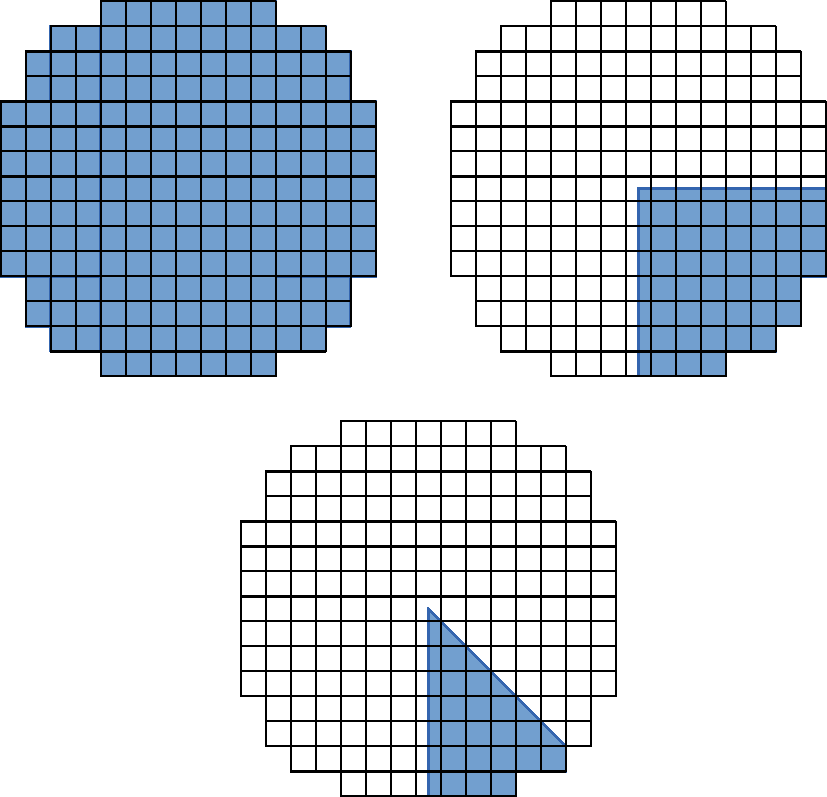
\includegraphics[width=5in]{figs/core_symmetry.pdf}
\end{center}
\caption{\label{fig:coresym} Full, quarter, and octant symmetry regions for a core map.}
\end{figure}

All of the maps require one entry for each assembly location defined in the {\it core\_shape} map.
However, the input parser can be used to take advantage of core symmetry.  If the core is symmetric,
you only need to input the maps in quarter or octant symmetry, and the input parser will automatically
fold the map out to full-symmetry.
The method used to input the core maps is independent of how the actual calculations are run.
For example, you can enter all of the core maps in octant symmetry and still run the calculations in quarter
or full symmetry.
The quadrant and octant that the parser is expecting is shown in Figure~\ref{fig:coresym}.

If there is an empty location in the map (e.g. if there is no detector or no control rod
in an assembly), enter a dash ``-''.  The dash is significant and signifies a blank location
in the core map.

\clearpage

The {\it assm\_map} shows where the assembly types are located within the core.
In the example below, there are three assembly types which will be defined in [ASSEMBLY] block(s).
\begin{verbatim}
  assm_map
                  A3 A3 A3 A3 A3 A3 A3
            A3 A3 A3 A1 A3 A1 A3 A1 A3 A3 A3
         A3 A3 A2 A1 A2 A1 A2 A1 A2 A1 A2 A3 A3
         A3 A2 A2 A2 A1 A2 A1 A2 A1 A2 A2 A2 A3
      A3 A3 A1 A2 A1 A2 A1 A2 A1 A2 A1 A2 A1 A3 A3
      A3 A1 A2 A1 A2 A1 A2 A1 A2 A1 A2 A1 A2 A1 A3
      A3 A3 A1 A2 A1 A2 A1 A2 A1 A2 A1 A2 A1 A3 A3
      A3 A1 A2 A1 A2 A1 A2 A1 A2 A1 A2 A1 A2 A1 A3
      A3 A3 A1 A2 A1 A2 A1 A2 A1 A2 A1 A2 A1 A3 A3
      A3 A1 A2 A1 A2 A1 A2 A1 A2 A1 A2 A1 A2 A1 A3
      A3 A3 A1 A2 A1 A2 A1 A2 A1 A2 A1 A2 A1 A3 A3
         A3 A2 A2 A2 A1 A2 A1 A2 A1 A2 A2 A2 A3
         A3 A3 A2 A1 A2 A1 A2 A1 A2 A1 A2 A3 A3
            A3 A3 A3 A1 A3 A1 A3 A1 A3 A3 A3
                  A3 A3 A3 A3 A3 A3 A3
\end{verbatim}

The following map is equivalent to the previous map, but demonstrates a map with octant symmetry.
Only values in the octant shown in Figure~\ref{fig:coresym} are entered and the parser automatically
folds the map out to full-symmetry.
\begin{verbatim}
  assm_map
     A1
     A2 A1
     A1 A2 A1
     A2 A1 A2 A1
     A1 A2 A1 A2 A2
     A2 A1 A2 A1 A2 A3
     A1 A3 A1 A3 A3 A3
     A3 A3 A3 A3         ! assembly map with octant symmetry
\end{verbatim}

The {\it insert\_map} is used to show where assembly inserts are located within the core.
In the following qtr-symmetry example,
the inserts are burnable poison assemblies with different numbers of pyrex rods.
The {\it insert\_map} can also be used to define thimble plug locations.
The geometry description of the inserts will be given in the [INSERT] block.
\begin{verbatim}
  insert_map
      -    BP20   -    BP20   -    BP20   -    BP12
     BP20   -    BP24   -    BP20   -    BP24   -
      -    BP24   -    BP20   -    BP16   -    BP8
     BP20   -    BP20   -    BP20   -    BP16   -
      -    BP20   -    BP20   -    BP24   -
     BP20   -    BP16   -    BP24  BP12   -
      -    BP24   -    BP16   -     -
     BP12   -    BP8    -
\end{verbatim}
The {\it insert\_map} is optional if no inserts are present in the core.
A dash ``-'' is used to specify assembly locations without an insert.

The {\it det\_map} is used to shows where detectors are located in the core.  The geometry description
of the detector strings is given in the [DETECTOR] block.  In this example,
there is only one detector type denoted with a ``1''.  Since the ``1'' occurs in a core map,
it is treated as a character string.  This example uses a full-symmetry map.
\begin{verbatim}
  det_map
                 -  -  1  -  -  1  -
           1  -  -  1  -  1  -  -  -  -  -
        -  -  -  -  -  -  1  -  1  -  1  -  1
        1  1  -  -  -  -  1  -  -  -  -  -  -
     -  -  -  -  1  -  -  -  1  -  1  -  1  -  -
     1  -  1  -  -  1  -  1  -  -  -  -  -  1  -
     -  -  -  1  -  -  1  -  -  1  -  -  1  -  -
     1  -  1  -  1  -  1  -  -  1  -  1  1  1  -
     -  1  -  -  -  -  -  -  1  -  1  -  -  -  1
     -  -  -  -  1  -  1  -  -  -  -  1  -  -  -
     1  -  -  -  1  -  -  1  -  -  1  -  -  -  1
        -  -  -  -  1  -  -  1  -  -  1  -  -
        -  1  -  1  -  -  1  -  -  -  -  -  1
           1  -  -  -  1  -  -  1  -  1  -
                 1  -  -  1  -  -  -
\end{verbatim}
The {\it det\_map} is optional if no detectors are present in the core.
A dash ``-'' is used to specify assembly locations without a detector.

% fix: Need to define what a control rod bank is

The control rod assemblies are described with two maps.  The {\it crd\_map}
defines the control rod types and locations in the core.
The {\it crd\_bank} map assigns control rod locations to control rod banks.
The control rod maps are optional if no control rods are present in the core.
\begin{verbatim}
  crd_map
                 -  -  -  -  -  -  -
           -  1  -  1  -  1  -  1  -  1  -
        -  -  -  1  -  1  -  1  -  1  -  -  -
        1  -  1  -  -  -  1  -  -  -  1  -  1
     -  -  1  -  1  -  -  -  -  -  1  -  1  -  -
     -  1  -  -  -  1  -  1  -  1  -  -  -  1  -
     -  -  1  -  -  -  -  -  -  -  -  -  1  -  -
     -  1  -  1  -  1  -  1  -  1  -  1  -  1  -
     -  -  1  -  -  -  -  -  -  -  -  -  1  -  -
     -  1  -  -  -  1  -  1  -  1  -  -  -  1  -
     -  -  1  -  1  -  -  -  -  -  1  -  1  -  -
        1  -  1  -  -  -  1  -  -  -  1  -  1
        -  -  -  1  -  1  -  1  -  1  -  -  -
           -  1  -  1  -  1  -  1  -  1  -
                 -  -  -  -  -  -  -
  crd_bank
                 -  -  -  -  -  -  -
           - SA  -  B  -  C  -  B  - SA  -
        -  -  - SD  - SB  - SB  - SC  -  -  -
       SA  -  D  -  -  -  D  -  -  -  D  - SA
     -  - SC  -  A  -  -  -  -  -  A  - SD  -  -
     -  B  -  -  -  C  -  A  -  C  -  -  -  B  -
     -  - SB  -  -  -  -  -  -  -  -  - SB  -  -
     -  C  -  D  -  A  -  D  -  A  -  D  -  C  -
     -  - SB  -  -  -  -  -  -  -  -  - SB  -  -
     -  B  -  -  -  C  -  A  -  C  -  -  -  B  -
     -  - SD  -  A  -  -  -  -  -  A  - SC  -  -
       SA  -  D  -  -  -  D  -  -  -  D  - SA
        -  -  - SC  - SB  - SB  - SD  -  -  -
           - SA  -  B  -  C  -  B  - SA  -
                 -  -  -  -  -  -  -

\end{verbatim}

%%%%%%%%%%%%%%%%%%%%%%%%%%%%%%%%%%%%%%%
\subsection{Core Baffle and Vessel}

The core baffle (sometimes called the shroud) is a steel reflector that closely surrounds
the fuel assemblies. The barrel is a round steel structure that surrounds the baffle, and
the vessel is the round outer pressure vessel.  These structures are shown in
Figure~\ref{fig:corebaffle}.

\begin{figure}
\begin{center}
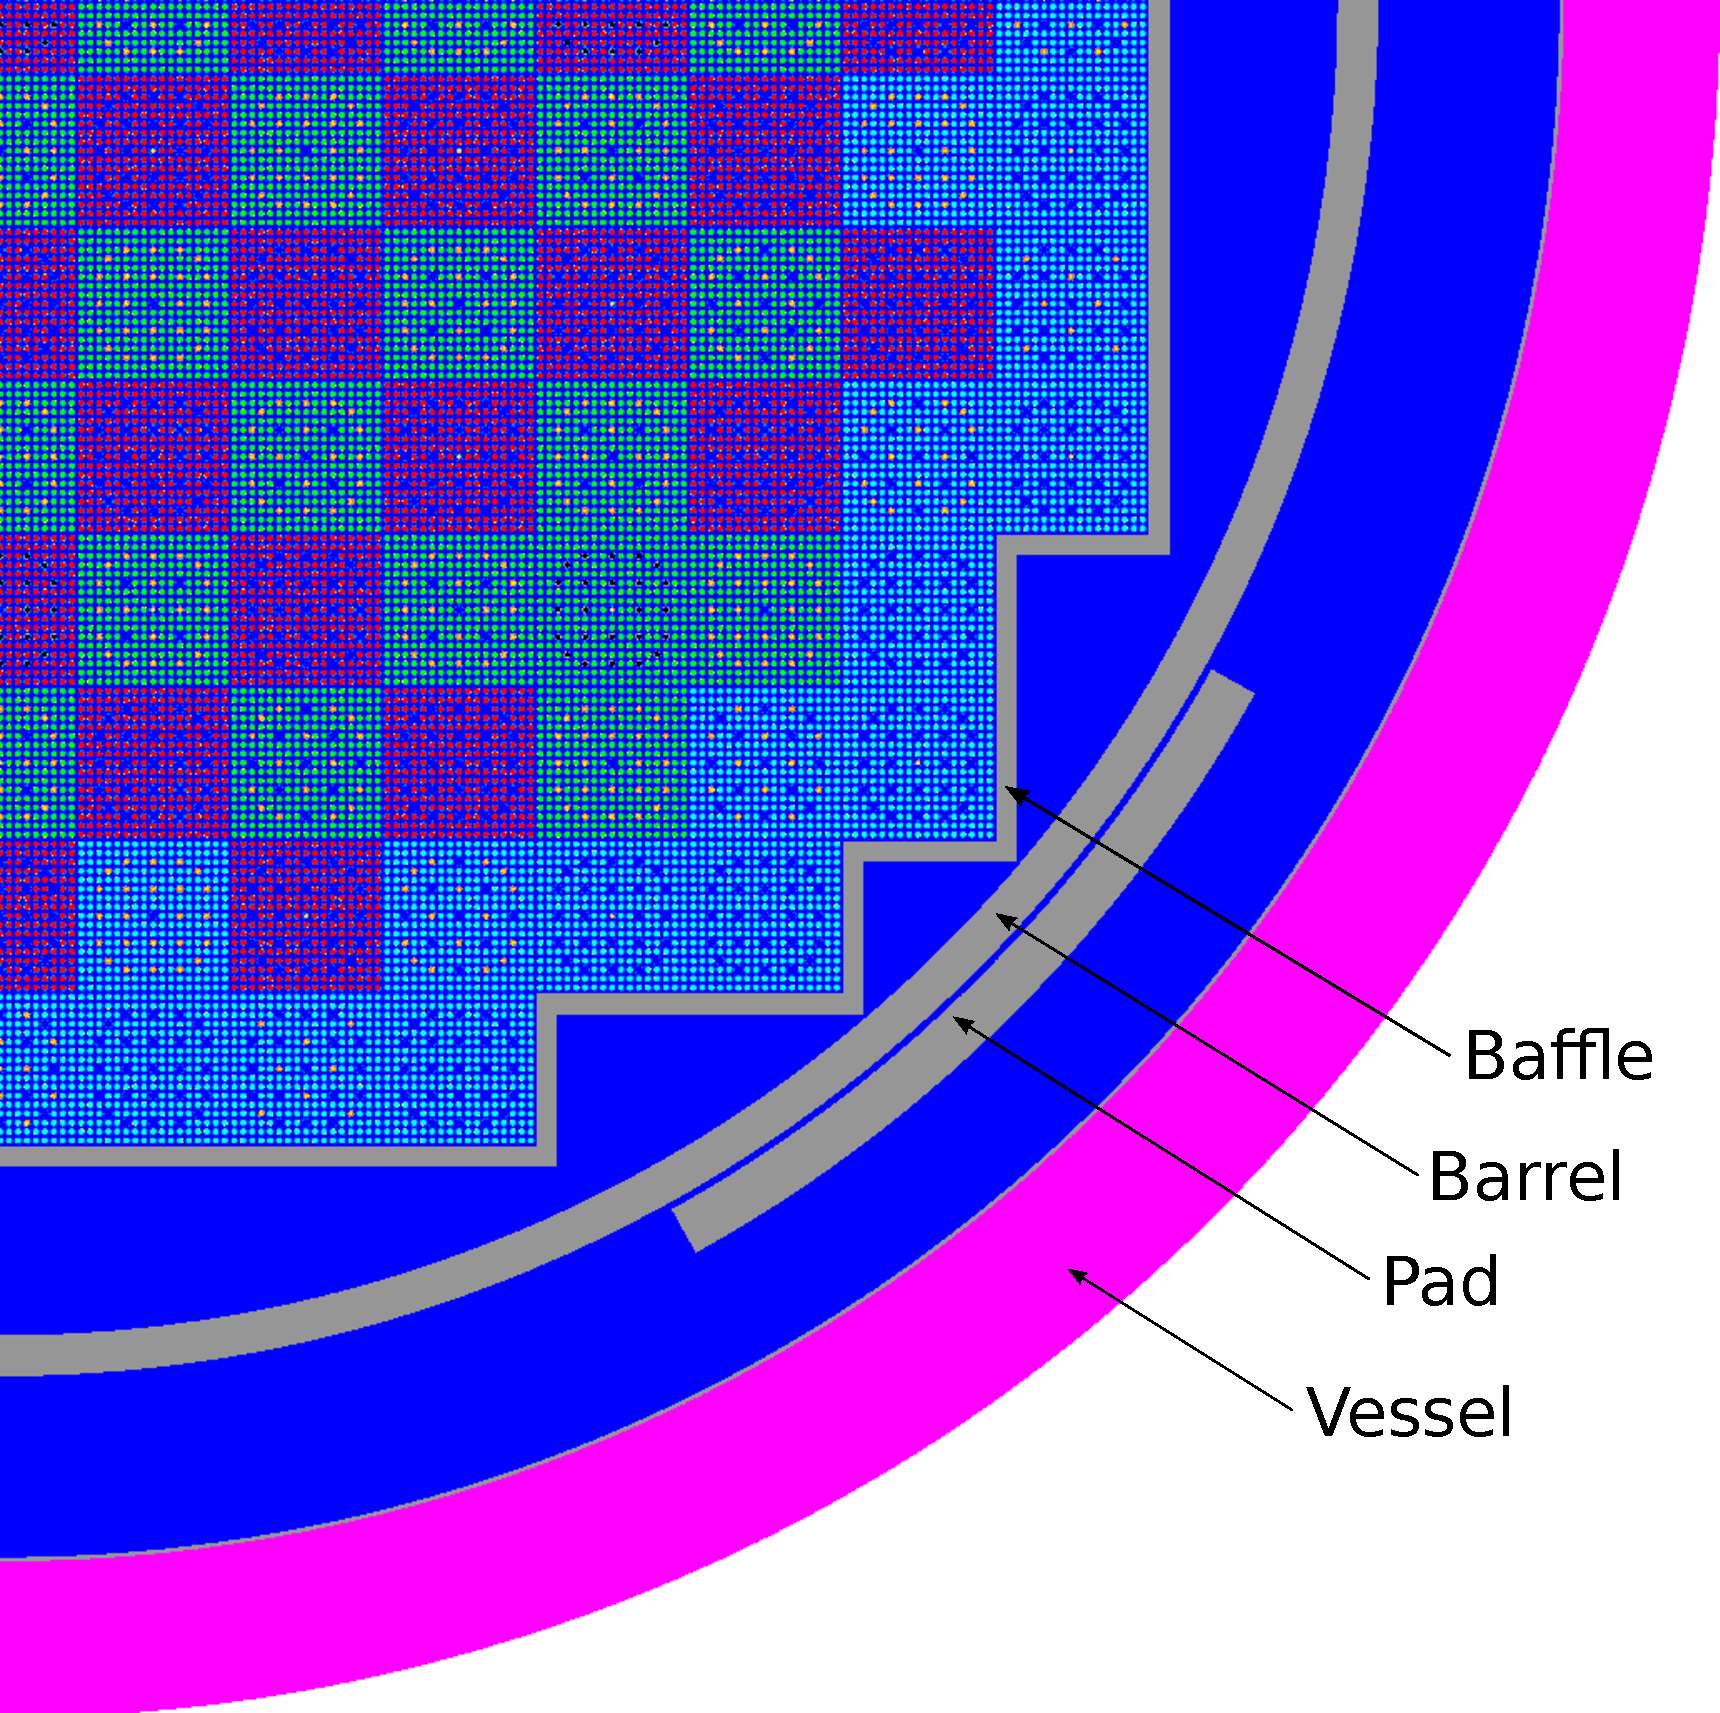
\includegraphics[width=5in]{figs/core_baffle.pdf}
\end{center}
\caption{\label{fig:corebaffle} Core baffle and vessel (image courtesy of Andrew Godfrey).}
\end{figure}

% fix: add figure showing exactly how the baffle gap is defined

The {\it baffle} is defined with a material, the size of the gap between the
outer assembly and baffle, and the baffle thickness.

The barrel and vessel are defined with a {\it vessel} card.  This card allows the
user to enter any arbitrary number of rings surrounding a core by specifying the
ring radii and the materials between the rings.

\begin{verbatim}
  baffle   SS304 0.19 1.26   ! material, gap (cm), and thickness (cm)
  vessel   mod 166.7 SS304 169.2 mod 175.0 SS304 176.0   ! materials and radii (cm)
\end{verbatim}

There is currently no input model for the neutron pad.

%%%%%%%%%%%%%%%%%%%%%%%%%%%%%%%%%%%%%%%
\subsection{Core Plates}

The core plates are large steel plates at the top and bottom of the core that have
various flow holes passing through it.  All of the core dimensions are relative to the
top of the bottom core plate and the total core {\it height} is defined as the distance
between the top of the bottom core plate and the bottom of the top core plate.

The core plates are modeled in the neutronics codes as smeared materials.
The upper and lower core plates are defined with a material composition, a thickness, and a
volume fraction of the structural material.
The remainder of the volume fraction is filled with coolant.

\begin{verbatim}
  lower_plate SS304  5.0  0.5   ! material, thickness (cm), volume fraction
  upper_plate SS304  7.6  0.5   ! material, thickness (cm), volume fraction
\end{verbatim}

%%%%%%%%%%%%%%%%%%%%%%%%%%%%%%%%%%%%%%%
\subsection{Small Cores Geometries}

Even though the VERA input is designed for ``real'' core geometries, it can accommodate smaller
problems as well.
For example, if you only want to run a single-assembly calculation, you would define the core size
as one assembly by one assembly, and all of the core maps would contain a single assembly.
\begin{verbatim}
  size 1                ! core composed of a single-assembly
  core_shape
     1
\end{verbatim}

If you want to model a single fuel rod, you would define a core with one assembly in it and
an assembly with one rod in it.



%%%%%%%%%%%%%%%%%%%%%%%%%%%%%%%
%  Section: Assemblies
%*-------------------------------------------------------------------------*
%*                 Copyright 2013 Core Physics, Inc.                       *
%*  Under terms of the contract to support CASL, there is a non-exclusive  *
%*  license for use of this work by or on behalf of the U.S. Government.   *
%*-------------------------------------------------------------------------*
%
% @version CVS $Id: assemblies.tex,v 1.8 2013/11/19 17:28:03 scott Exp $
%
%%%%%%%%%%%%%%%%%%%%%%%%%%%%%%%%%%%%%%%%%%%%%%%%%%%%%%%%%%%%%%%%
\section{Assembly Description}

The [ASSEMBLY] block contains the geometric description of a unique fuel assembly.
Multiple [ASSEMBLY] blocks are allowed to described different assembly designs in the core.

If there are multiple assembly designs that are geometrically identical (i.e. everything is the same except
the enrichments), then they can all be defined in a single [ASSEMBLY] block.
Each assembly type will have a unique {\it axial} card with possibly unique axial levels and lattice types.
Assemblies within a single reload typically have a design similar enough that they can share a single
[ASSEMBLY] block.

If assembly designs are not geometrically identical (e.g. different vendors, different generations, etc.)
they need to be defined in separate [ASSEMBLY] blocks.
One advantage to having separate blocks for each assembly design is that each design can be
modeled (and archived) independently without having to rely on global definitions.

A typical PWR assembly is shown in Figure~\ref{fig:assembly}.  Refer to this figure in the following discussions.
\begin{figure}
\begin{center}
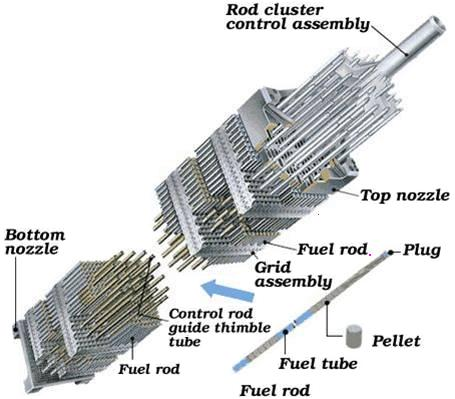
\includegraphics[width=4in]{figs/PWR-assembly.jpg}
\end{center}
\caption{\label{fig:assembly} PWR Fuel Assembly (source: Public internet).}
\end{figure}

%%%%%%%%%%%%%%%%%%%%%%%%%%%
\subsection{Initial Data}

Each assembly must contain a geometry description with the number of pins across the assembly and
the pin pitch.  An assembly block can also include an optional title card.
\begin{verbatim}
  title "Westinghouse 17x17"      ! assembly title
  npin 17                         ! number of pins across one side
  ppitch 1.260                    ! pin pitch (cm)
\end{verbatim}

The number of pins {\it npin} must be the same for every assembly in a core.

The inter-assembly gap on each side of the assembly is calculated with $[apitch-npin*ppitch]/2$

The fuel and structural materials are defined with the following cards.
See Chapter~\ref{chap:materials} for a complete description of the material inputs.
\begin{verbatim}
  fuel U31 10.257 95.0 / 3.1   ! mat, density (g/cc), Theoretical density (%)
                               !    / U-235 enrichment (%)
  mat inc  8.19                ! mat, density (g/cc)
  mat ss   8.0
  mat zirc 6.56
\end{verbatim}

%%%%%%%%%%%%%%%%%%%%%%%%%%%
\subsection{Cell Descriptions}

Cell cards are used to describe ``pincells''.  Pincells are usually defined as fuel rods or guide tubes
surrounded by a square region of coolant, however, the definitions are general so they can be used
to describe any configuration of of concentric cylindars (or rings) surrounded by a square region
filled with coolant.  
Figure~\ref{fig:pincell} shows a pincell configuration for a fuel rod and a guide tube.
\begin{figure}
\begin{center}
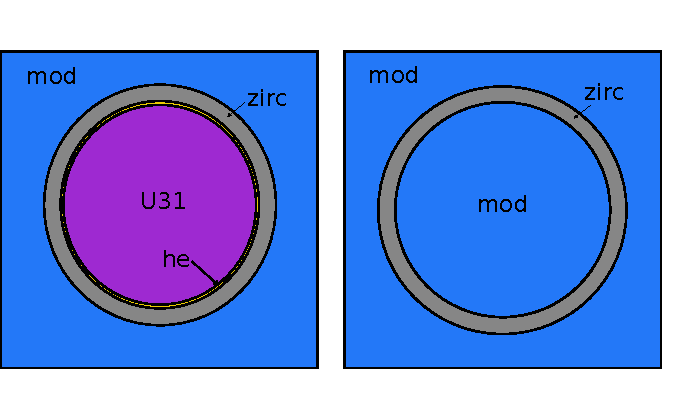
\includegraphics[width=4in]{figs/pincell1.pdf}
\end{center}
\caption{\label{fig:pincell} Pincell diagrams of a fuel rod and a guide tube.}
\end{figure}

The first parameter on the {\it cell} card is the cell ID.
This is followed by a list of radii for each ring in the pincell, followed by a slash.
After the slash is a list of materials that go into each ring.
The cell ID's are used in the lattice descriptions described in the next section.

\begin{verbatim}
  cell 1     0.4096 0.418 0.475 / U31 he zirc
  cell GT           0.561 0.602 / mod    zirc       ! guide tube
  cell IT           0.561 0.602 / mod    zirc       ! instrument tube
  cell 7            0.418 0.475 / mod    mod        ! empty location
  cell 8            0.418 0.475 /     he zirc       ! plenum
  cell 9                  0.475 /        zirc       ! pincap
\end{verbatim}

In this example, in cell 1, the material ``U31'' extends from radius 0 to 0.4096.
The material ``he'' extends from a radius 0.4096 to 0.418.
The definition of materials ``U31'' and ``he'' are defined on {\it fuel} and {\it mat} cards, respectively.
(Material cards are described in Chapter~\ref{chap:materials}.)

The outside of each pincell is automatically filled with the special material ``mod'', which
refers to the moderator (or coolant).
The composition of ``mod'' is calculated by the local T/H conditions and the soluble boron concentration,
and cannot be specified by a user on a {\it mat} card.

In the example above, the guide tube (GT) and instrument tube (IT) descriptions
use the special moderator material ``mod'' to define the moderator material on both
the inside and outside of the guide tubes.

%%%%%%%%%%%%%%%%%%%%%%%%%%%
\subsection{Lattice Descriptions}

Once the cells are defined, they are placed into 2D ``lattices'' as shown below.
Like the core maps, the lattice maps can be entered with either full-symmetry, qtr-symmetry,
or octant-symmetry.  The maps below are octant symmetric maps for 17x17 assembly designs.

\begin{verbatim}
  lattice FUEL1
      IT
       1 1
       1 1 1
      GT 1 1 GT
       1 1 1  1 1
       1 1 1  1 1 GT
      GT 1 1 GT 1  1 1
       1 1 1  1 1  1 1 1
       1 1 1  1 1  1 1 1 1

  lattice LGAP1
      IT
       7 7
       7 7 7
      GT 7 7 GT
       7 7 7  7 7
       7 7 7  7 7 GT
      GT 7 7 GT 7  7 7
       7 7 7  7 7  7 7 7
       7 7 7  7 7  7 7 7 7

  lattice PLEN1
      IT
       8 8
       8 8 8
      GT 8 8 GT
       8 8 8  8 8
       8 8 8  8 8 GT
      GT 8 8 GT 8  8 8
       8 8 8  8 8  8 8 8
       8 8 8  8 8  8 8 8 8

  lattice PCAP1
      IT
       9 9
       9 9 9
      GT 9 9 GT
       9 9 9  9 9
       9 9 9  9 9 GT
      GT 9 9 GT 9  9 9
       9 9 9  9 9  9 9 9
       9 9 9  9 9  9 9 9 9
\end{verbatim}

Lattice cards define each unique axial level in the assembly.
The first parameter is the lattice name (e.g. FUEL1, PCAP1, etc.),
followed by a map of the {\it cell} ID's.

%%%%%%%%%%%%%%%%%%%%%%%%%%%
\subsection{Axial Descriptions}

After lattice maps are defined for each axial level, the lattices are ``stacked'' into
an assembly using {\it axial} cards as shown below.

\begin{verbatim}
  axial A1    6.050
      LGAP1  10.281
      PCAP1  11.951
      FUEL1 377.711
      PLEN1 393.711
      PCAP1 395.381
      LGAP1 397.501
\end{verbatim}

The {\it axial} card tells the code how to place the lattices axially.
The first parameter is the name of the assembly (A1), followed by a
list of elevations and lattice types.
For example, lattice ``FUEL1'' extends from 11.951 to 377.711 cm axially.

If multiple assembly types are defined in one [ASSEMBLY] block, there will be
multiple {\it axial} cards, each with a unique assembly ID.

All elevations are defined relative to the top of the lower core plate.

%%%%%%%%%%%%%%%%%%%%%%%%%%%
\subsection{Grid Spacer Descriptions}

Grid cards are used to define unique grid spacer types.
The following example defines two grid types, ``END'' and ``MID''.

\begin{verbatim}
  grid END inc  1017  3.866   ! grid spacer material, mass(kg), height(cm)
  grid MID zirc  875  3.810
\end{verbatim}

The grid types are placed axially with the {\it grid\_axial} card:
\begin{verbatim}
  grid_axial
      END  13.884
      MID  75.2
      MID 127.4
      MID 179.6
      MID 231.8
      MID 284.0
      MID 336.2
      END 388.2
\end{verbatim}

The elevations are the midpoints of the spacer grid and are relative to the top of the lower core plate.

%%%%%%%%%%%%%%%%%%%%%%%%%%%
\subsection{Nozzle Descriptions}

The assembly nozzles are modeled in the neutronics codes as smeared materials.  This is a very good
approximation since the nozzles are not in the active fuel region and are mostly
composed of water, steel, and zirconium.  The user only specifies a nozzle mass and a nozzle height.
The total volume of the nozzle region is calculated from the assembly pitch and nozzle height.
The volume of the nozzle is calculated from the nozzle mass and density.
The volume of the coolant is then calculated as the total volume minus the volume of the nozzle.
The coolant density is updated with the local T/H conditions.

% A typical PWR assembly nozzle is shown in Figure~\ref{fig:nozzle}.
% \begin{figure}
% \begin{center}
% 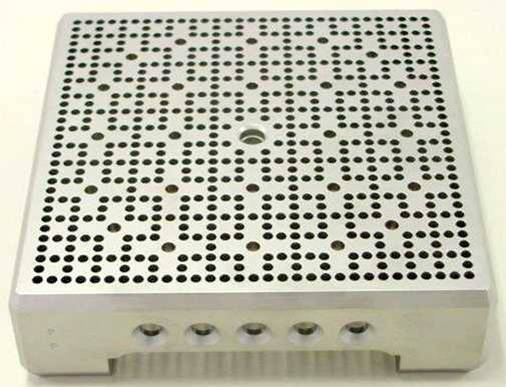
\includegraphics[width=4in]{figs/nozzle.jpg}
% \end{center}
% \caption{\label{fig:nozzle} PWR Assembly Lower Nozzle.}
% \end{figure}

\begin{verbatim}
  lower_nozzle  ss 6.05  6250.0  ! mat, height, mass (g)
  upper_nozzle  ss 8.827 6250.0  ! mat, height, mass (g)
\end{verbatim}

Note that the {\it lower\_nozzle} height should match the bottom elevation on the {\it axial} card.
The {\it upper\_nozzle} height + the top elevation on the {\it axial} card must match the
core {\it height} in the [CORE] block.
The input parser does not currently perform a check to make sure the elevations are consistent.
Therefore, this check should be performed in each of the individual physics codes.

%%%%%%%%%%%%%%%%%%%%%%%%%%%%%%%%%%%%%%%%%%%%%%%%%%%%%%%%%%%
\section{Control Rod Assembly Description}

The [CONTROL] block contains the geometric description of a control assembly.

A control rod assembly is defined in the same way as a fuel assembly is described.
You define cells, lattices, and axial descriptions.  The only difference between
the control rod assembly and the fuel assembly is that the control rod assembly
describes what is inside the guide tubes and the fuel assembly description defines the
guide tubes themselves.

The geometric description for a control rod is given in the {\bf fully inserted} position.

\begin{verbatim}
  title "B4C control rods with AIC tips"   ! control_title
  npin 17                                  ! control_num_pins

  cell 1  0.382 0.386 0.484 / aic he ss      ! AIC cell
  cell 2  0.373 0.386 0.484 / b4c he ss      ! B4C cell

  rodmap  AIC
     -
     - -
     - - -
     1 - - 1
     - - - - -
     - - - - - 1
     1 - - 1 - - -
     - - - - - - - -
     - - - - - - - - -

  rodmap  B4C
     -
     - -
     - - -
     2 - - 2
     - - - - -
     - - - - - 2
     2 - - 2 - - -
     - - - - - - - -
     - - - - - - - - -

  axial CR1 15.76 AIC  376.44 B4C  394.3
\end{verbatim}

Note that the name of the control rod ``CR1'' refers to the control rod type in the
{\it crd\_map} in the [CORE] block.

Note that the locations of the control rod fingers must match the guide tube locations in the
corresponding [ASSEMBLY] block descriptions.  Furthermore, the outer radii of the control
rod fingers must be smaller than the inner radii of the guide tubes.
The input parser does not currently perform a check to make sure the control rod finger
descriptions are consistent with the guide tube descriptions.
This check should be performed in each of the individual physics codes.

The user can define materials in the [CONTROL] block.  These materials only have scope in
this block and are not accessible by other blocks.  See Chapter~\ref{chap:materials} for details.

%%%%%%%%%%%%%%%%%%%%%%%%%%%
\subsection{Control Rod Stroke}

One difference between the control rod description and the assembly description is that
the control rod moves during operation and the movement must be defined with a {\it stroke} card.

The first value on the {\it stroke} card is the total length of the control rod travel (stroke)
from fully inserted to fully withdrawn.

The second value on the {\it stroke} card is the number of steps in the fully withdrawn position.
Step 0 is the fully inserted position.
\begin{verbatim}
  stroke  360.0 228      ! stroke (cm), number of steps fully withdrawn
\end{verbatim}

All elevations given in the geometric description are for a control rod in the
fully inserted position (step 0).

\subsection{Control Rod Position Example}

From the {\it axial} card shown above, the bottom of the AIC at the fully-inserted position is 15.46 cm.
From the {\it stroke} card, the total stroke is 360.0 cm and the number of steps in the fully withdrawn
position is 228 steps.
Therefore, the bottom elevation of the AIC lattice at step N will be
\begin{equation}
   E(N) = 15.46 + \frac{360.0 \cdot N}{228}
\end{equation}

Using this formula, the bottom elevation of the AIC lattice at the following step positions is:
\begin{itemize}   % itemize = bullet list
 \item step 228 (fully withdrawn)= 15.46 + 360.0 * 228 / 228 = 375.46 cm
 \item step 100 = 15.46 + 360.0 * 100 / 228 = 173.35 cm
 \item step 0 (fully inserted) = 15.46 + 360.0 * 0 / 228 = 15.46 cm
\end{itemize}

%%%%%%%%%%%%%%%%%%%%%%%%%%%%%%%%%%%%%%
\section{Insert Description}
An assembly insert is defined in the same way as a fuel assembly or control rod assembly is described.
You define the insert using cells, lattices, and axial descriptions.

The only difference between an assembly insert and the fuel assembly description is that assembly insert
describes what is inside the guide tubes and the assembly description defines the
guide tubes themselves.

The following example shows a definition of a Pyrex insert.

\begin{verbatim}
[INSERT]
    title "Pyrex"
    npin 17
    mat pyrx1 2.25 pyrex-vera
    cell 1  0.214 0.231 0.241 0.427 0.437 0.484 / he ss he pyrx1 he ss
    rodmap  PY24
       -
       - -
       - - -
       1 - - 1
       - - - - -
       - - - - - 1
       1 - - 1 - - -
       - - - - - - - -
       - - - - - - - - -

    axial INS24  15.76 PY24 376.441
\end{verbatim}

The name of the insert ``INS24'' refers to an insert type defined in the
{\it insert\_map} in the [CORE] block.

The locations of the insert fingers must match the guide tube locations in the
corresponding [ASSEMBLY] block descriptions.  Furthermore, the outer radii of the insert
fingers must be smaller than the inner radii of the guide tubes.
The input parser does not currently perform a check to make sure the insert finger
descriptions are consistent with the guide tube descriptions.
This check should be performed in each of the individual physics codes.

%%%%%%%%%%%%%%%%%%%%%%%%%%%%%%%%%%%%%%
\section{Detector Description}
A detector string is defined in the same way that a fuel assembly is described.
You define cells, lattices, and axial descriptions to define the detector string.

\begin{verbatim}
  [DETECTOR]
    title "Incore instrument thimble"
    npin 17

    mat he 0.0001786
    mat ss 8.0

    cell 1  0.258 0.382 / he ss

    rodmap  LAT
       1
       - -
       - - -
       - - - -
       - - - - -
       - - - - - -
       - - - - - - -
       - - - - - - - -
       - - - - - - - - -

    axial D1  0.0 LAT 406.337
\end{verbatim}





%%%%%%%%%%%%%%%%%%%%%%%%%%%%%%%
\section{Statepoint Values}

The [STATE] block defines the state of the core at a particular point in time
(power, flow, pressure, inlet temperature, rod positions, boron concentration, etc.).
These values will typically change during a depletion.

An example showing the most common input cards in the [STATE] block is shown below.

\begin{verbatim}
  [STATE]
    power   98.0       ! % of rated power
    flow   100.0       ! % of rated flow
    pressure 2250.0    ! psia
    tinlet 557.33      ! F
    feedback on        ! turn on T/H feedback

    boron  1285        ! initial boron ppmB
    search 'boron'     ! turn on boron search

    sym qtr            ! run problem in qtr-symmetry

    rodbank SA 228
            SB 228
            SC 228
            SD 228
             A 228
             B 228
             C 228
             D 167
\end{verbatim}

The {\it sym} card tells the code to run the calculation in full-core symmetry or
qtr-core symmetry. If the calculation is run in qtr-core symmetry, the symmetry is either
set to qtr-core rotational or qtr-core mirror by the {\it bc\_sym} card in the [CORE] block.

The {\it rodbank} card is used to position the control rods. The input includes pairs of bank names
and bank positions.  The bank names correspond to the {\it crd\_map} in the [CORE] block.
The positions indicate the position of the control rod bank in steps.
For most PWR's, 0 steps is fully inserted.
The number of steps for a rod to be completely withdrawn is set by the {\it stroke} card in
the [CONTROL] block. For Westinghouse PWR's, a typical value of fully-withdrawn is 228 steps.

%%%%%%%%%%%%%%%%%%%%%%%%%%%%%%%
\section{Edits}

The [EDITS] block is used to define the edits the user would like to see.

The {\it axial\_edit\_bounds} defines the axial levels to average the power over.
The user may choose to average power over uniform axial intervals (like most nodal codes),
or to specify the edit intervals manually.

\subsection{CTF Nodalization}

The [EDITS] block is also used to set the axial nodalization in CTF.

If running CTF, there is a restriction that the grid boundaries must be explicitly
included in the {\it axial\_edit\_bounds}. This can get a little complicated for the user.
The grids are defined by specifying the grid heights on the {\it grid} card and the elevations of
the grid midpoints on the {\it grid\_axial} card.
These heights and midpoints must be converted to the elevations at the top and bottom of the grid,
and then the top and bottom elevations must be included in the {\it axial\_edit\_bounds}.

For example, if a grid is defined with a centerline at 75.0 and a height of 2.5, then the
{\it axial\_edit\_bounds} must include the points $75.0 \pm 1.25 $= 73.75 and 76.25.

\begin{verbatim}
   [ASSEMBLY]
    grid GRID1 inc 1000 2.5    ! grid name, material, mass (g), and height (cm)
    grid_axial                 ! locations of grid midpoints (cm)
        GRID1 75.0

   [EDITS]
    axial_edit_bounds
       ...
       73.75                   ! this array must include top and bottom grid boundaries
       76.25
       ...
\end{verbatim}

The reason for this restriction is because the power is already calculated on the {\it axial\_edit\_bounds},
so it is natural to use these boundaries in the CTF model as well.
The grids must be explicitly included in the CTF boundaries so the loss coefficients are calculated correctly.

In the future, this restriction may be lifted and an additional edit bounds array will
be added explicitly for CTF calculations.


%%%%%%%%%%%%%%%%%%%%%%%%%%%%%%%
\section{Coupling Parameters}

The [COUPLING] block defines the relaxation parameters and convergence criteria to be
used when coupling different physics codes.  These values are used to determine
convergence {\it between} physics codes.  Convergence criteria {\it within} a physics
code is controlled by the specific code block.

Refer to Chapter \ref{chap:cards} for a complete listing of all the cards in the [COUPLING] block.

No code-specific information is included in the [COUPLING] block.  All code-specific information
is contained in the code-specific blocks.

As an example, consider the following multi-physics code coupling:
\begin{enumerate}
  \item  Run T/H calculation
  \item  Run neutronics calculation
  \item  Check eigenvalue convergence \label{stepepsk}
  \item  Check power convergence \label{stepepsp}
  \item  Relax/dampen the power shape
  \item  If not converged, go to step 1.
\end{enumerate}
The eigenvalue convergence in step \ref{stepepsk} uses the parameter {\it epsk} to check
the change in eigenvalue between coupled iterations.
There are additional eigenvalue convergence criteria {\it within} the neutronics
code, but the internal parameters are specified in the individual code blocks.

The power convergence in step \ref{stepepsp} uses the parameter {\it epsp} to check
the change in power between coupled iterations.

Additional convergence checks are made on the peak fuel temperature, maximum change in density,
and change in boron concentration (if applicable).

The example shown above uses a Picard iteration to converge.  Picard iterations usually
need to apply a relaxation factor (also called a damping factor or under-relaxation factor) to
one or more of the calculated quantities to converge.
The relaxation factors are applied in the following manner:
\begin{equation}
  x = \omega \, x^{\mbox{new}} + (1 - \omega) x^{\mbox{old}}
\end{equation}
where $x$ is the calculated parameter and $\omega$ is the relaxation factor.
A relaxation factor of 1.0 signifies no relaxation is performed.
A relaxation factor $< 1.0$ signifies under-relaxation.

Relaxation factors can be specified for the point-wise power, point-wise temperature, and/or point-wise density.
The relaxation is applied to the transferred quantities sent between physics codes.  The state variables
within each physics code are not changed.


%%%%%%%%%%%%%%%%%%%%%%%%%%%%%%%%%%%%%%%%%
%  Chapter: Materials
%*-------------------------------------------------------------------------*
%*                 Copyright 2013 Core Physics, Inc.                       *
%*  Under terms of the contract to support CASL, there is a non-exclusive  *
%*  license for use of this work by or on behalf of the U.S. Government.   *
%*-------------------------------------------------------------------------*
%
% @version CVS $Id: materials.tex,v 1.11 2013/11/19 17:28:04 scott Exp $
%
%%%%%%%%%%%%%%%%%%%%%%%%%%%%%%%%%%%%%%%%%
\chapter{Materials Description}  \label{chap:materials}

This chapter contains a description of the material input.  There are two types of materials
in the input file -- structural materials (input with a {\it mat} card) and fuel materials
(input with a {\it fuel} card).

Structural materials can be defined in either the [CORE] block, or in the
geometry object blocks [ASSEMBLY], [INSERT], [CONTROL], and [DETECTOR].
If the materials are defined in the [CORE] block, they have global scope.
If the materials are defined in the geometry object blocks, they only have
scope in the block they are defined.
The reason for this is to maintain the modularity of the geometry objects.

Fuel materials can only be defined in [ASSEMBLY] blocks.

Materials are used in many different input cards.  They are used to define
cells, nozzles, core plates, baffles, grids, reflectors, etc.  Every material that
is used must be defined with either a {\it mat} card or a {\it fuel} card.

%%%%%%%%%%%%%%%%%%%%%%%%%%%%%%%%
\section{Structural Materials}

Structural materials are not fuel and do not deplete.  Structural
materials are defined with the following input card:

{\bf mat} {\it user-mat} {\it density} ({\it library-name$_i$}, {\it frac$_i$}, i=1, I)

where:
\begin{itemize}
\item {\it user-mat} is a user-defined material name.  It is case sensitive.  {\it user-mat} is used to
define material names in other input cards such as {\it cell}, {\it grid}, {\it nozzle}, etc. (No default)
\item {\it density} is the material density in g/cc (No default)
\item {\it library-name} is a corresponding material library name for the user material.  The library name
must be defined in the material composition file. (Default = {\it user-mat}).  Multiple library materials
can be mixed to form a single user material.
\item {\it frac}  is the fraction of the library material in the user material. (Default=1.0 if there is only one library material in the user material).
\end{itemize}

There are two special user materials,  ``mod'' and ``vacuum''.
The user can use these materials in cell definitions, but the code will be automatically
determine the composition of these materials  based on T/H feedback and soluble boron concentrations.
The user is not allowed to define a user materials named ``mod'' or ``vacuum'' on a {\it mat} card.

Some example material cards are shown below.
\begin{verbatim}
  mat zirc 6.56                ! use default library name and fraction
  mat zirc 6.56 zirc4 1.0
  mat B10  12.0 boron 1.0
  mat XYZ  6.0  zirc4 0.8 ss 0.2
  mat ABCD 8.0  zirc4 0.8 ss 0.15 b4c 0.05
\end{verbatim}

All of the material fractions must sum to either +1.0 or -1.0.
If positive fractions are used, the fractions refer to atomic fractions.
If negative fractions are used, the fractions refer to weight fractions.


%%%%%%%%%%%%%%%%%%%%%%
\subsection{Search Order}

Structural materials can be defined in either the [CORE] block or one of the
geometry object blocks.  When a material is referred to in a block, it will look
for the material definition in the following order:
\begin{enumerate}  % enumerate = numbered list
 \item The code will first look for the material name in the local block ([ASSEMBLY], [INSERT], [CONTROL], or [DETECTOR])
 \item If the material is not found in the local block, it will look in the [CORE] block
\end{enumerate}

If materials are defined in the [CORE] block, they have global scope over the entire input.
If materials are defined in other blocks, they only have scope over the local block.  This means
that two geometry object blocks can use different material definitions with the same name.
One example of this is that two assemblies can be defined with the material ``zirc'', but
the ``zirc'' can have different compositions in the blocks.

%%%%%%%%%%%%%%%%%%%%%%%%%%
\section{Composition File}

All library materials must be included in the HDF composition file.
The name of the composition file is specified on the [INSILICO] {\it mat\_library} card,
or the [MPACT] {\it (TBD)} card, and is usually named something like ``casl\_comp.sh5''.

A partial list of materials that are present on the current composition file is:
\begin{itemize}   % itemize = bullet list
  \item aic
  \item b4c
  \item boron
  \item inc
  \item he
  \item mod
  \item ss
  \item zirc
\end{itemize}


%%%%%%%%%%%%%%%%%%%%%%%%
\section{Fuel Materials}

Fuel materials are composed mostly of UO$_2$ with different U-235 enrichments.
Fuel materials are different from structural materials in that they deplete and have
additional properties as described below.

Fuel can only be defined in [ASSEMBLY] blocks, and fuel materials can only be referenced by {\it cell} cards
in the [ASSEMBLY] block they are defined in.

Fuel materials are defined with the following input card:

{\bf fuel} {\it user-mat} {\it density} {\it thden} / {\it U-235\_enrichment} \{{\it HM\_material$_i$}={\it HM\_enrichment$_i$}, i=1, N\}  \\
   \{ / {\it gad\_material}={\it gad\_fraction} \}

Where:

\begin{itemize}   % itemize = bullet list
  \item {\it user-mat} is a user-defined fuel name. It is case sensitive. (No default)
  \item {\it density} is the fuel material density in g/cc (No default)
  \item {\it thden} is the percent of theoretical density in the pellet (\%) (No default)
  \item {\it U-235\_enrichment} is the U-235 enrichment in the fuel in weight \%  (No default).
  \begin{itemize}   % itemize = bullet list
    \item If U-234 and U-236 are not specified, the enrichments will automatically be added to the
       fuel by a pre-determined function (see below)
    \item If the sum of the heavy metal (HM) enrichments does not equal 100\%, the remainder of the
        HM composition will be assigned to U-238.
  \end{itemize}
  \item {\it HM\_material$_i$} is the material name for a HM (Pu-239, Pu-241, etc.) (optional)
  \item {\it HM\_enrichment$_i$} is the enrichment of HM isotope $i$ in weight \% (optional)
  \item {\it gad\_material} is the material name for the gad oxide (or other material) (optional).
        The gad material may be a mixture defined on a separate {\it mat} card.
  \item {\it gad\_fraction} is the weight percent of the gad material relative to the total mass (optional)
\end{itemize}

Oxygen should not be included on the {\it fuel} card.  The correct amount of oxygen will automatically
be added to the HM to create an oxide (either UO$_2$  or (HM)O$_2$).

The {\it density} is the ``stack density'' or ``smeared density'' and should include the volume
of the pellet dishing and chamfers.
It is calculated as the total mass of the fuel pellets divided by the total volume of the fuel
\begin{equation}
  \mbox{stack density} = \frac{ (\mbox{fuel mass})} { \pi (\mbox{pellet radius})^2 \, (\mbox{fuel height}) }
\end{equation}

The {\it thden} refers to the actual density of the pellet.  This quantity is
only used in fuel performance codes to evaluate material properties.

If U-234 or U-236 enrichments are not included, they are automatically added to the fuel with the following formulas:
\begin{equation}
   W_{234} = 0.007731 \cdot W_{235}^{1.0837}
\end{equation}
\begin{equation}
  W_{236} = 0.0046 \cdot W_{235}
\end{equation}
Where $W_{23x}$ is the enrichment of each of the uranium isotopes in percent.


Examples of valid fuel cards are:
\begin{verbatim}
  fuel U21 10.4 95.2 / 2.1
  fuel UO2-35 10.297 95.0 / 3.5
  fuel U23 10.111 / 2.3                      ! bare minimum input for fuel
  mat gad5 7.407 gd2o3 1.0                   ! define gad material
  fuel U49 10.111 94.5 / 1.8  / gad5=0.05    ! 5% gad
  fuel PX1 10.111 94.5 / 0.711  Pu-239=23.4  Pu-241=1.9    ! Sample MOX
  fuel UPX21G 10.111 94.5 / 2.1 U-234=0.001 Pu-239=3.4  Pu-241=1.9 / gad3=0.03
\end{verbatim}





%%%%%%%%%%%%%%%%%%%%%%%%%%%%%%%%%%%%%%%%%
\chapter{Input Card Descriptions} \label{chap:cards}
This chapter contains a complete listing of the available input cards.

The input for each block is given in a separate subsection.

Input cards are given in {\bf bold} text followed by the parameters on the card.
Following each input card is a description of the parameters on that card.

An example of an input card is:

{\bf card\_name} param1, param2
\begin{cardlist}
  \item[param1]  The first parameter on card (units)
  \item[param2]  The second parameter on card (units)
\end{cardlist}


%*-------------------------------------------------------------------------*
%*                 Copyright 2013 Core Physics, Inc.                       *
%*  Under terms of the contract to support CASL, there is a non-exclusive  *
%*  license for use of this work by or on behalf of the U.S. Government.   *
%*-------------------------------------------------------------------------*
%
% WARNING: This file is autogenerated, do not modify by hand!
%
%%%%%%%%%%%%%%%%%%%%%%%%%%%%%%%%%%%%%%%%%%%%%%%
\section{Block CASEID}

{\bf [CASEID]}

{\bf title} case\_id
\begin{cardlist}
  \item[case\_id]  Problem name
\end{cardlist}

%%%%%%%%%%%%%%%%%%%%%%%%%%%%%%%%%%%%%%%%%%%%%%%
\section{Block STATE}

{\bf [STATE]}

{\bf title} title
\begin{cardlist}
  \item[title]  Statepoint title
\end{cardlist}

{\bf power} power
\begin{cardlist}
  \item[power]  Operating power (percent of rated power)
\end{cardlist}

{\bf flow} flow
\begin{cardlist}
  \item[flow]   Operating flow  (percent of rated flow)
\end{cardlist}

{\bf bypass} bypass
\begin{cardlist}
  \item[bypass]  Bypass flow (percent of rated flow)
\end{cardlist}

{\bf tinlet} tinlet
\begin{cardlist}
  \item[tinlet]  Inlet temperature (degrees F**)
\end{cardlist}

{\bf tfuel} tfuel
\begin{cardlist}
  \item[tfuel]  Fixed fuel temperatures (degrees K) - Only used without T/H feedback
\end{cardlist}

{\bf modden} modden
\begin{cardlist}
  \item[modden]  Fixed moderator density (g/cc) - Only used without T/H feedback
\end{cardlist}

{\bf xenon} xenopt
\begin{cardlist}
  \item[xenopt]  Xenon option (``zer'', ``dep'', or ``equil'')
\end{cardlist}

{\bf samar} sampot
\begin{cardlist}
  \item[sampot]  Samarium option (``zer'', ``dep'', ``equil'', or ``peak'')
\end{cardlist}

{\bf boron} boron
\begin{cardlist}
  \item[boron]  Soluble boron concentration (ppm)
\end{cardlist}

{\bf kcrit} kcrit
\begin{cardlist}
  \item[kcrit]  Critical eigenvalue used in boron search
\end{cardlist}

{\bf search} search
\begin{cardlist}
  \item[search]  Search option (``keff'' or ``boron'')
\end{cardlist}

{\bf pressure} pressure
\begin{cardlist}
  \item[pressure]  Core exit pressure (psia)
\end{cardlist}

{\bf deplete} deplete
\begin{cardlist}
  \item[deplete]  List of depletion exposure steps (MWD/MTU) - only used with depletion
\end{cardlist}

{\bf rodbank} bank\_pos, bank\_labels
\begin{cardlist}
  \item[bank\_pos]  Steps withdrawn for each bank in list
  \item[bank\_labels]  List of control rod banks to position.  Labels correspond to crd\_map in CORE block.
\end{cardlist}

{\bf feedback} feedback
\begin{cardlist}
  \item[feedback]  Flag to turn on and off T/H feedback (``on'' or ``off'').  Currently not used, feedback is controlled by executable that is run.
\end{cardlist}

{\bf sym} sym
\begin{cardlist}
  \item[sym]  Core fraction to run problem in (``full'' or ``qtr'')
\end{cardlist}

%%%%%%%%%%%%%%%%%%%%%%%%%%%%%%%%%%%%%%%%%%%%%%%
\section{Block CORE}

{\bf [CORE]}

{\bf name} core\_name
\begin{cardlist}
  \item[core\_name]  Name of the reactor core
\end{cardlist}

{\bf cycle} cycle\_num, cyc\_stdate, cyc\_edate
\begin{cardlist}
  \item[cycle\_num]  Cycle number
  \item[cyc\_stdate]  Cycle startup date (YYYYMMDD)
  \item[cyc\_edate]  Cycle end date (YYYYMMDD).  Enter zero if end date is not known.
\end{cardlist}

{\bf size} core\_size
\begin{cardlist}
  \item[core\_size]  Number of assemblies across one axis in full-core geometry (required)
\end{cardlist}

{\bf rated} rated\_power, rated\_flow
\begin{cardlist}
  \item[rated\_power]  Rated thermal power at 100\% power (MW)
  \item[rated\_flow]   Rated vessel flow at 100\% flow (Mlbs/hr**)
\end{cardlist}

{\bf apitch} apitch
\begin{cardlist}
  \item[apitch]  Assembly pitch (cm)
\end{cardlist}

{\bf baffle} baffle\_mat, baffle\_gap, baffle\_thick
\begin{cardlist}
  \item[baffle\_mat]   Baffle material
  \item[baffle\_gap]   Gap between outside assembly (including assembly gap) and baffle (cm)
  \item[baffle\_thick]   Thickness of baffle (cm)
\end{cardlist}

{\bf vessel} vessel\_mats, vessel\_radii
\begin{cardlist}
  \item[vessel\_mats]  Vessel materials
  \item[vessel\_radii]  Vessel radii (cm)
\end{cardlist}

{\bf core\_shape} shape
\begin{cardlist}
  \item[shape]  Square map showing the fuel assembly locations.  Enter 1 for fuel assembly locations and 0 for empty locations.
\end{cardlist}

{\bf assm\_map} assm\_map
\begin{cardlist}
  \item[assm\_map]  Core map of the fuel assembly types.  The assembly types correspond to assembly labels in the ASSEMBLY block.  All fuel assemblies must have a type defined.
\end{cardlist}

{\bf insert\_map} insert\_map
\begin{cardlist}
  \item[insert\_map]  Core map of the fuel insert types and locations.  The insert types correspond to insert labels in the INSERT block.  Use a dash to specify assemblies with no inserts.
\end{cardlist}

{\bf det\_map} det\_map
\begin{cardlist}
  \item[det\_map]  Core map of the detector types and locations.  The detector types correspond to detector labels in the DETECTOR block.  Use a dash to specify assemblies with no detectors.
\end{cardlist}

{\bf crd\_map} crd\_map
\begin{cardlist}
  \item[crd\_map]  Core map of the control rod types and locations.  The control rod types correspond to control rod labels in the CONTROL block.  Use a dash to specify assemblies with no control rods.
\end{cardlist}

{\bf crd\_bank} crd\_bank
\begin{cardlist}
  \item[crd\_bank]  Core map of the control rod bank labels.  These labels are used to position groups of control rods by bank label.  Use a dash to specify assemblies with no control rods.
\end{cardlist}

{\bf lower\_plate} lower\_mat, lower\_thick, lower\_vfrac
\begin{cardlist}
  \item[lower\_mat]  Lower core plate material
  \item[lower\_thick]  Lower core plate thickness (cm)
  \item[lower\_vfrac]  Lower core plate volume fraction.  Remainder of volume fraction will be filled with coolant.
\end{cardlist}

{\bf upper\_plate} upper\_mat, upper\_thick, upper\_vfrac
\begin{cardlist}
  \item[upper\_mat]  Upper core plate material
  \item[upper\_thick]  Upper core plate thickness (cm)
  \item[upper\_vfrac]  Upper core plate volume fraction.  Remainder of volume fraction will be filled with coolant.
\end{cardlist}

{\bf bc\_sym} bc\_sym
\begin{cardlist}
  \item[bc\_sym]  Symmetry flag for the core when using qtr-symmetry.  Flag is not used in full-symmetry.  Valid  options are ``rot'' and ``mir''.
\end{cardlist}

{\bf bc\_bot} bc\_bot
\begin{cardlist}
  \item[bc\_bot]  Bottom neutron transport boundary condition, ``vacuum'' (default) or ``reflecting''.
\end{cardlist}

{\bf bc\_top} bc\_top
\begin{cardlist}
  \item[bc\_top]  Top neutron transport boundary condition, ``vacuum'' (default) or ``reflecting''.
\end{cardlist}

{\bf bc\_rad} bc\_rad
\begin{cardlist}
  \item[bc\_rad]  Radial neutron transport boundary condition, ``vacuum'' (default) or ``reflecting''.
\end{cardlist}

{\bf xlabel} xlabel
\begin{cardlist}
  \item[xlabel]  List of 2-character assembly position labels in x-direction.  These values are used in the edit maps.
\end{cardlist}

{\bf ylabel} ylabel
\begin{cardlist}
  \item[ylabel]  List of 2-character assembly position labels in y-direction.  These values are used in the edit maps.
\end{cardlist}

{\bf height} height
\begin{cardlist}
  \item[height]  Total axial distance from bottom core plate to upper core plate (cm).  Distance does not include core plate thicknesses.
\end{cardlist}

{\bf mat} mat
\begin{cardlist}
  \item[mat]  See detailed Materials description.
\end{cardlist}

{\bf lower\_ref} lower\_refl\_mats, lower\_refl\_thicks, lower\_refl\_vfracs
\begin{cardlist}
  \item[lower\_refl\_mats]  Lower reflector materials
  \item[lower\_refl\_thicks]  Lower reflector thicknesses (cm)
  \item[lower\_refl\_vfracs]  Lower reflector volume fractions
\end{cardlist}

{\bf upper\_ref} upper\_refl\_mats, upper\_refl\_thicks, upper\_refl\_vfracs
\begin{cardlist}
  \item[upper\_refl\_mats]  Upper reflector materials
  \item[upper\_refl\_thicks]  Upper reflector thicknesses (cm)
  \item[upper\_refl\_vfracs]  Upper reflector volume fractions
\end{cardlist}

%%%%%%%%%%%%%%%%%%%%%%%%%%%%%%%%%%%%%%%%%%%%%%%
\section{Block ASSEMBLY}

{\bf [ASSEMBLY]}

{\bf title} title
\begin{cardlist}
  \item[title]  Long descriptive title for assembly.
\end{cardlist}

{\bf npin} num\_pins
\begin{cardlist}
  \item[num\_pins]  The number of rods along the edge of an assembly.
\end{cardlist}

{\bf ppitch} ppitch
\begin{cardlist}
  \item[ppitch]  Cell pitch (cm)
\end{cardlist}

{\bf cell} cell
\begin{cardlist}
  \item[cell]  Refer to the cell description given in the User's Manual.
\end{cardlist}

{\bf lattice} axial\_label, cell\_map
\begin{cardlist}
  \item[axial\_label]  Label for this axial elevation description.
  \item[cell\_map]  Lattice map for this axial elevation.  Use a dash for an empty location.
\end{cardlist}

{\bf axial} label, axial\_labels, axial\_elevations
\begin{cardlist}
  \item[label]  Label for this assembly.  Label corresponds to assm\_map in CORE block.
  \item[axial\_labels]  List of axial labels for this assembly description.  Corrrespond to labels in lattice maps.
  \item[axial\_elevations]  List of axial elevations for this assembly description (cm).
\end{cardlist}

{\bf dancoff} dancoff\_map
\begin{cardlist}
  \item[dancoff\_map]  Lattice map of dancoff factors (not currently used in the calculation).
\end{cardlist}

{\bf grid} label, material, mass, height
\begin{cardlist}
  \item[label]  Grid label for a single grid type.
  \item[material]  Grid material for this grid type.
  \item[mass]      Grid mass for this grid type (g).
  \item[height]    Grid height for this grid type (cm).
\end{cardlist}

{\bf grid\_axial} grid\_map, grid\_elev
\begin{cardlist}
  \item[grid\_map]   List of spacer grid labels for all grids in an assembly (labels correspond to grid card)
  \item[grid\_elev]  List of spacer grid elevations for all grids in an assembly (cm).  Elevations refer to the grid midpoint.
\end{cardlist}

{\bf lower\_nozzle} lower\_nozzle\_comp, lower\_nozzle\_height, lower\_nozzle\_mass
\begin{cardlist}
  \item[lower\_nozzle\_comp]  Lower nozzle material.
  \item[lower\_nozzle\_height]  Lower nozzle height (cm)
  \item[lower\_nozzle\_mass]  Lower nozzle mass (g).  Code will calculate the volume of the nozzle given the nozzle mass, and use coolant for remaining volume.
\end{cardlist}

{\bf upper\_nozzle} upper\_nozzle\_comp, upper\_nozzle\_height, upper\_nozzle\_mass
\begin{cardlist}
  \item[upper\_nozzle\_comp]  Upper nozzle material.
  \item[upper\_nozzle\_height]  Upper nozzle height (cm)
  \item[upper\_nozzle\_mass]  Upper nozzle mass (g).  Code will calculate the volume of the nozzle given the nozzle mass, and use coolant for remaining volume.
\end{cardlist}

{\bf fuel} fuel
\begin{cardlist}
  \item[fuel]  See detailed Materials description.
\end{cardlist}

{\bf mat} mat
\begin{cardlist}
  \item[mat]  See detailed Materials description.
\end{cardlist}

%%%%%%%%%%%%%%%%%%%%%%%%%%%%%%%%%%%%%%%%%%%%%%%
\section{Block CONTROL}

{\bf [CONTROL]}

{\bf title} title
\begin{cardlist}
  \item[title]  Long descriptive title for control rod description.
\end{cardlist}

{\bf npin} num\_pins
\begin{cardlist}
  \item[num\_pins]  The number of rods along the edge of an assembly.
\end{cardlist}

{\bf stroke} stroke, maxstep
\begin{cardlist}
  \item[stroke]  Control rod stroke - distance between full-insertion and full-withdrawal (cm)
  \item[maxstep]  Total number of steps between full-insertion and full-withdrawal
\end{cardlist}

{\bf cell} Cell
\begin{cardlist}
  \item[Cell]   Refer to the cell description given in the User's Manual.
\end{cardlist}

{\bf rodmap} label, cell\_map
\begin{cardlist}
  \item[label]  Label for this axial elevation description
  \item[cell\_map]  Lattice map for this axial elevation.  Use a dash for no control rod.
\end{cardlist}

{\bf axial} control\_label, axial\_labels, axial\_elevations
\begin{cardlist}
  \item[control\_label]  Label for this control rod description.  Label corresponds to crd\_map in CORE block.
  \item[axial\_labels]  List of axial labels for this control rod description.  Corrrespond to labels in rod maps.
  \item[axial\_elevations]  List of axial elevations for this control rod description (cm).
\end{cardlist}

{\bf mat} mat
\begin{cardlist}
  \item[mat]  See detailed Materials description.
\end{cardlist}

%%%%%%%%%%%%%%%%%%%%%%%%%%%%%%%%%%%%%%%%%%%%%%%
\section{Block INSERT}

{\bf [INSERT]}

{\bf title} title
\begin{cardlist}
  \item[title]  Long descriptive title for assembly insert description.
\end{cardlist}

{\bf npin} num\_pins
\begin{cardlist}
  \item[num\_pins]  The number of rods along the edge of an assembly.
\end{cardlist}

{\bf cell} Cell
\begin{cardlist}
  \item[Cell]   Refer to the cell description given in the User's Manual.
\end{cardlist}

{\bf rodmap} label, cell\_map
\begin{cardlist}
  \item[label]  Label for this axial elevation description
  \item[cell\_map]  Lattice map for this axial elevation. Use a dash for no insert rod.
\end{cardlist}

{\bf axial} insert\_label, axial\_labels, axial\_elevations
\begin{cardlist}
  \item[insert\_label]  Label for this assembly insert description.  Label corresponds to insert\_map in CORE block.
  \item[axial\_labels]  List of axial labels for this assembly insert description.  Corrrespond to labels in rod maps.
  \item[axial\_elevations]  List of axial elevations for this assembly insert description (cm).
\end{cardlist}

{\bf mat} mat
\begin{cardlist}
  \item[mat]  See detailed Materials description.
\end{cardlist}

%%%%%%%%%%%%%%%%%%%%%%%%%%%%%%%%%%%%%%%%%%%%%%%
\section{Block DETECTOR}

{\bf [DETECTOR]}

{\bf title} title
\begin{cardlist}
  \item[title]  Long descriptive title for detector description.
\end{cardlist}

{\bf npin} num\_pins
\begin{cardlist}
  \item[num\_pins]  The number of rods along the edge of an assembly.
\end{cardlist}

{\bf cell} Cell
\begin{cardlist}
  \item[Cell]   Refer to the cell description given in the User's Manual.
\end{cardlist}

{\bf rodmap} label, cell\_map
\begin{cardlist}
  \item[label]  Label for this axial elevation description
  \item[cell\_map]  Lattice map for this axial elevation. Use a dash for no detector rod.
\end{cardlist}

{\bf axial} detector\_label, axial\_labels, axial\_elevations
\begin{cardlist}
  \item[detector\_label]  Label for this detector description.  Label corresponds to det\_map in CORE block.
  \item[axial\_labels]  List of axial labels for this detector description.  Corrrespond to labels in rod maps.
  \item[axial\_elevations]  List of axial elevations for this detector description (cm).
\end{cardlist}

{\bf mat} mat
\begin{cardlist}
  \item[mat]  See detailed Materials description.
\end{cardlist}

%%%%%%%%%%%%%%%%%%%%%%%%%%%%%%%%%%%%%%%%%%%%%%%
\section{Block EDITS}

{\bf [EDITS]}

{\bf axial\_edit\_bounds} axial\_edit\_bounds
\begin{cardlist}
  \item[axial\_edit\_bounds]   The boundaries of the axial regions over which axial information should be printed.
\end{cardlist}

{\bf axial\_edit\_mesh\_delta} axial\_edit\_mesh\_delta
\begin{cardlist}
  \item[axial\_edit\_mesh\_delta]  Produces a uniform axial output grid (integrates pin powers over a uniform axial mesh).
\end{cardlist}

%%%%%%%%%%%%%%%%%%%%%%%%%%%%%%%%%%%%%%%%%%%%%%%
\section{Block COBRATF}

{\bf [COBRATF]}

{\bf nfuel} nfuel
\begin{cardlist}
  \item[nfuel]  Number of radial nodes in fuel pellet.
\end{cardlist}

{\bf nc} nc
\begin{cardlist}
  \item[nc]  Conduction option (see CTF manual).
\end{cardlist}

{\bf irfc} irfc
\begin{cardlist}
  \item[irfc]  Friction factor correlation number (see CTF manual).
\end{cardlist}

{\bf dhfrac} dhfrac
\begin{cardlist}
  \item[dhfrac]  Fraction of power deposited directly in coolant.
\end{cardlist}

{\bf hgap} hgap
\begin{cardlist}
  \item[hgap]  Gap conductance (W/m$^2$ K)
\end{cardlist}

{\bf gridloss} gridlabel, gridloss
\begin{cardlist}
  \item[gridlabel]  Spacer grid label (from ASSEMBLY block).
  \item[gridloss]  Spacer grid loss coefficient.
\end{cardlist}

{\bf epso} epso
\begin{cardlist}
  \item[epso]  Outer iteration convergence criteria.
\end{cardlist}

{\bf oitmax} oitmax
\begin{cardlist}
  \item[oitmax]  Maximum number of outer iterations.
\end{cardlist}

{\bf iitmax} iitmax
\begin{cardlist}
  \item[iitmax]  Maximum number of vessel iterations
\end{cardlist}

{\bf dtmin} dtmin
\begin{cardlist}
  \item[dtmin]  Minimum time step (s).
\end{cardlist}

{\bf dtmax} dtmax
\begin{cardlist}
  \item[dtmax]  Maximum time step (s).
\end{cardlist}

{\bf tend} tend
\begin{cardlist}
  \item[tend]  End of time domain (s).
\end{cardlist}

{\bf rtwfp} rtwfp
\begin{cardlist}
  \item[rtwfp]  Ratio of time step sizes for conduction/fluid.
\end{cardlist}

{\bf maxits} maxits
\begin{cardlist}
  \item[maxits]  Maximum number of iterations.
\end{cardlist}

{\bf courant} courant
\begin{cardlist}
  \item[courant]  Courant limit
\end{cardlist}

{\bf maps\_filename} maps\_filename
\begin{cardlist}
  \item[maps\_filename]   ??
\end{cardlist}

{\bf heated\_elements\_type} heated\_elements\_type
\begin{cardlist}
  \item[heated\_elements\_type]  ??
\end{cardlist}

{\bf heater\_tube\_id} heater\_tube\_id
\begin{cardlist}
  \item[heater\_tube\_id]  ??
\end{cardlist}

{\bf heater\_tube\_od} heater\_tube\_od
\begin{cardlist}
  \item[heater\_tube\_od]  ??
\end{cardlist}

{\bf heater\_tube\_pitch} heater\_tube\_pitch
\begin{cardlist}
  \item[heater\_tube\_pitch]  ??
\end{cardlist}

{\bf solver} solver
\begin{cardlist}
  \item[solver]  ??
\end{cardlist}

{\bf parallel} parallel
\begin{cardlist}
  \item[parallel]  0=serial execution, 1=parallel exectution.  Parallelization is on a per-assembly basis.
\end{cardlist}

{\bf global\_energy\_balance} global\_energy\_balance
\begin{cardlist}
  \item[global\_energy\_balance]  Convergence criteria
\end{cardlist}

{\bf global\_mass\_balance} global\_mass\_balance
\begin{cardlist}
  \item[global\_mass\_balance]  Convergence criteria
\end{cardlist}

{\bf fluid\_energy\_storage} fluid\_energy\_storage
\begin{cardlist}
  \item[fluid\_energy\_storage]  Convergence criteria
\end{cardlist}

{\bf solid\_energy\_storage} solid\_energy\_storage
\begin{cardlist}
  \item[solid\_energy\_storage]  Convergence criteria
\end{cardlist}

{\bf mass\_storage} mass\_storage
\begin{cardlist}
  \item[mass\_storage]  Convergence criteria
\end{cardlist}

%%%%%%%%%%%%%%%%%%%%%%%%%%%%%%%%%%%%%%%%%%%%%%%
\section{Block COUPLING}

{\bf [COUPLING]}

{\bf epsk} epsk
\begin{cardlist}
  \item[epsk]  Eigenvalue converence criteria (pcm)
\end{cardlist}

{\bf epsp} epsp
\begin{cardlist}
  \item[epsp]  Power convergence criteria (L2 norm)
\end{cardlist}

{\bf eps\_temp} eps\_temp
\begin{cardlist}
  \item[eps\_temp]  Temperature convergence criteria (degrees F)
\end{cardlist}

{\bf eps\_boron} eps\_boron
\begin{cardlist}
  \item[eps\_boron]  Boron convergence criteria (ppm)
\end{cardlist}

{\bf rlx\_power} rlx\_power
\begin{cardlist}
  \item[rlx\_power]  Power relaxation factor.  Recommend 0.5.
\end{cardlist}

{\bf rlx\_tfuel} rlx\_tfuel
\begin{cardlist}
  \item[rlx\_tfuel]  Fuel temperature relaxation factor.  Recommend 1.0.
\end{cardlist}

{\bf rlx\_den} rlx\_den
\begin{cardlist}
  \item[rlx\_den]  Density relaxation factor.  Recommend 1.0.
\end{cardlist}

{\bf maxiter} maxiter
\begin{cardlist}
  \item[maxiter]  Maximum number of coupled iterations.
\end{cardlist}

{\bf read\_restart} read\_restart
\begin{cardlist}
  \item[read\_restart]  Name of restart file.  Leave blank for no restart.
\end{cardlist}

{\bf LIME\_xml} LIME\_xml
\begin{cardlist}
  \item[LIME\_xml]    Name of LIME XML file.  The use of this card is deprecated, the LIME XML file is now created automatically.  See the LIME Users Manual for more information.
\end{cardlist}


%%%%%%%%%%%%%%%%%%%%%%%%%%%%%%%%%%%%%%%%%
\chapter{Example}

This chapter includes a complete input example for a full-core problem.
This problem is Problem 7 of the AMA Progression Benchmark Problems and
is based upon the publicly available description of the Watts Bar reactors.

%*-------------------------------------------------------------------------*
%*                 Copyright 2013-2015 Core Physics, Inc.                  *
%*  Under terms of the contract to support CASL, there is a non-exclusive  *
%*  license for use of this work by or on behalf of the U.S. Government.   *
%*-------------------------------------------------------------------------*
%
% @version CVS $Id: example.tex,v 1.9 2015/02/23 01:48:13 scott Exp $
%
% Example file
\begin{Verbatim}[fontsize=\small]
  !
  !  Sample Test case for Problem 7 (Full-Core HFP)
  !
  [CASEID]
    title 'CASL Progression Problem 7 - Watts Bar Unit 1 Cycle 1 - Public'

  [STATE]
    power  100.0          ! % of rated power
    flow   100.0          ! % of rated flow
    pressure 2250.0
    feedback on

    tinlet 565.0 K        !
    tfuel  900.0 K        ! (HFP value)
    boron  1285           ! ppmB
    modden 0.743          ! g/cc
    sym qtr

    rodbank SA 230
            SB 230
            SC 230
            SD 230
             A 230
             B 230
             C 230
             D 167

  [CORE]
    size 15               ! assemblies across core
    rated 3411 131.68     ! MW, Mlbs/hr
    apitch 21.5
    height 406.337

    core_shape
      0 0 0 0 1 1 1 1 1 1 1 0 0 0 0
      0 0 1 1 1 1 1 1 1 1 1 1 1 0 0
      0 1 1 1 1 1 1 1 1 1 1 1 1 1 0
      0 1 1 1 1 1 1 1 1 1 1 1 1 1 0
      1 1 1 1 1 1 1 1 1 1 1 1 1 1 1
      1 1 1 1 1 1 1 1 1 1 1 1 1 1 1
      1 1 1 1 1 1 1 1 1 1 1 1 1 1 1
      1 1 1 1 1 1 1 1 1 1 1 1 1 1 1
      1 1 1 1 1 1 1 1 1 1 1 1 1 1 1
      1 1 1 1 1 1 1 1 1 1 1 1 1 1 1
      1 1 1 1 1 1 1 1 1 1 1 1 1 1 1
      0 1 1 1 1 1 1 1 1 1 1 1 1 1 0
      0 1 1 1 1 1 1 1 1 1 1 1 1 1 0
      0 0 1 1 1 1 1 1 1 1 1 1 1 0 0
      0 0 0 0 1 1 1 1 1 1 1 0 0 0 0

    assm_map
      1
      2 1
      1 2 1
      2 1 2 1
      1 2 1 2 2
      2 1 2 1 2 3
      1 3 1 3 3 3
      3 3 3 3

    insert_map
       -
      20  -
       - 24  -
      20  - 20  -
       - 20  - 20  -
      20  - 16  - 24 12
       - 24  - 16  -  -
      12  -  8  -

    crd_map
      1
      - -
      1 - 1
      - - - 1
      1 - - - 1
      - 1 - 1 - -
      1 - 1 - 1 -
      - - - -

    crd_bank
      D  -  A  -  D  -  C  -
      -  -  -  -  - SB  -  -
      A  -  C  -  -  -  B  -
      -  -  -  A  - SC  -  -
      D  -  -  -  D  - SA
      - SB  - SD  -  -  -
      C  -  B  - SA  -
      -  -  -  -

    det_map
              1 - - 1 - - -
          1 - - - 1 - - 1 - 1 -
        - 1 - 1 - - 1 - - - - - 1
        - - - - 1 - - 1 - - 1 - -
      1 - - - 1 - - 1 - - 1 - - - 1
      - - - - 1 - 1 - - - - 1 - - -
      - 1 - - - - - - 1 - 1 - - - 1
      1 - 1 - 1 - 1 - - 1 - 1 1 1 -
      - - - 1 - - 1 - - 1 - - 1 - -
      1 - 1 - - 1 - 1 - - - - - 1 -
      - - - - 1 - - - 1 - 1 - 1 - -
        1 1 - - - - 1 - - - - - -
        - - - - - - 1 - 1 - 1 - 1
          1 - - 1 - 1 - - - - -
              - - 1 - - 1 -

    baffle ss 0.19 2.85
    vessel mod 219.71 cs 241.70

    lower_plate ss  5.0 0.5   ! mat, thickness, vol frac
    upper_plate ss  7.6 0.5   ! mat, thickness, vol frac

    lower_ref  mod 20.0 1.0   ! mat, thickness, vol frac
    upper_ref  mod 20.0 1.0   ! mat, thickness, vol frac

    xlabel  R P N M L K J H G  F  E  D  C  B  A
    ylabel  1 2 3 4 5 6 7 8 9 10 11 12 13 14 15

    mat he     0.0001786
    mat inc    8.19
    mat ss     8.0
    mat zirc   6.56 zirc4

  [ASSEMBLY]
    title "Westinghouse 17x17 Assembly"
    npin 17
    ppitch 1.260

    fuel U21 10.257 94.5 / 2.110
    fuel U26 10.257 94.5 / 2.619
    fuel U31 10.257 94.5 / 3.100

    cell 1     0.4096 0.418 0.475 / U21 he zirc
    cell 2     0.4096 0.418 0.475 / U26 he zirc
    cell 3     0.4096 0.418 0.475 / U31 he zirc
    cell 4            0.561 0.602 / mod    zirc       ! guide/instrument tube
    cell 5            0.418 0.475 /     he zirc       ! plenum

    rodmap LAT21
         4
         1 1
         1 1 1
         4 1 1 4
         1 1 1 1 1
         1 1 1 1 1 4
         4 1 1 4 1 1 1
         1 1 1 1 1 1 1 1
         1 1 1 1 1 1 1 1 1

    rodmap LAT26
         4
         2 2
         2 2 2
         4 2 2 4
         2 2 2 2 2
         2 2 2 2 2 4
         4 2 2 4 2 2 2
         2 2 2 2 2 2 2 2
         2 2 2 2 2 2 2 2 2

    rodmap LAT31
         4
         3 3
         3 3 3
         4 3 3 4
         3 3 3 3 3
         3 3 3 3 3 4
         4 3 3 4 3 3 3
         3 3 3 3 3 3 3 3
         3 3 3 3 3 3 3 3 3

    rodmap PLEN
         4
         5 5
         5 5 5
         4 5 5 4
         5 5 5 5 5
         5 5 5 5 5 4
         4 5 5 4 5 5 5
         5 5 5 5 5 5 5 5
         5 5 5 5 5 5 5 5 5

    axial  1  11.951 LAT21 377.711 PLEN 393.711
    axial  2  11.951 LAT26 377.711 PLEN 393.711
    axial  3  11.951 LAT31 377.711 PLEN 393.711

    grid END inc  1017 3.866
    grid MID zirc 875  3.810

    grid_axial
        END  13.884
        MID  75.2
        MID 127.4
        MID 179.6
        MID 231.8
        MID 284.0
        MID 336.2
        END 388.2

    lower_nozzle  ss 6.053 6250.0  ! mat, height, mass (g)
    upper_nozzle  ss 8.827 6250.0  ! mat, height, mass (g)

  [INSERT]
    title "Pyrex"
    npin 17

    mat pyrx1 2.25 pyrex-vera

    cell 1  0.214 0.231 0.241 0.427 0.437 0.484 / he ss he pyrx1 he ss

    rodmap  PY8
       -
       - -
       - - -
       1 - - -
       - - - - -
       - - - - - 1
       - - - - - - -
       - - - - - - - -
       - - - - - - - - -

    rodmap  PY12
       -
       - -
       - - -
       1 - - -
       - - - - -
       - - - - - -
       - - - 1 - - -
       - - - - - - - -
       - - - - - - - - -

    rodmap  PY16
       -
       - -
       - - -
       1 - - -
       - - - - -
       - - - - - 1
       - - - 1 - - -
       - - - - - - - -
       - - - - - - - - -

    rodmap  PY20
       -
       - -
       - - -
       1 - - -
       - - - - -
       - - - - - 1
       1 - - 1 - - -
       - - - - - - - -
       - - - - - - - - -

    rodmap  PY24
       -
       - -
       - - -
       1 - - 1
       - - - - -
       - - - - - 1
       1 - - 1 - - -
       - - - - - - - -
       - - - - - - - - -

    axial   8  15.761 PY8  376.441
    axial  12  15.761 PY12 376.441
    axial  16  15.761 PY16 376.441
    axial  20  15.761 PY20 376.441
    axial  24  15.761 PY24 376.441

  [CONTROL]
    title "B4C with AIC tips"
    npin 17
    stroke  365.125 230     ! approx for 1.5875 step sizes and 230 max stroke

    mat aic 10.2
    mat b4c 1.76

    cell 1  0.382 0.386 0.484 / aic he ss
    cell 2  0.373 0.386 0.484 / b4c he ss

    rodmap AIC
       -
       - -
       - - -
       1 - - 1
       - - - - -
       - - - - - 1
       1 - - 1 - - -
       - - - - - - - -
       - - - - - - - - -

    rodmap B4C
       -
       - -
       - - -
       2 - - 2
       - - - - -
       - - - - - 2
       2 - - 2 - - -
       - - - - - - - -
       - - - - - - - - -

    axial  1    17.031
           AIC 118.631
           B4C 377.711

  [DETECTOR]
    title "Incore instrument thimble"
    npin 17

    mat he 0.0001786
    mat ss 8.0

    cell 1  0.258 0.382 / he ss

    rodmap  LAT
       1
       - -
       - - -
       - - - -
       - - - - -
       - - - - - -
       - - - - - - -
       - - - - - - - -
       - - - - - - - - -

    axial 1  0.0 LAT 406.337

  [EDITS]
    axial_edit_bounds
         11.951   15.817   24.028   32.239   40.45
         48.662   56.873   65.084   73.295   77.105
         85.17    93.235  101.3    109.365  117.43
        125.495  129.305  137.37   145.435  153.5
        161.565  169.63   177.695  181.505  189.57
        197.635  205.7    213.765  221.83   229.895
        233.705  241.77   249.835  257.9    265.965
        274.03   282.095  285.905  293.97   302.035
        310.1    318.165  326.23   334.295  338.105
        346.0262 353.9474 361.8686 369.7898 377.711

  [COBRATF]
    nfuel   10            ! number of fuel rings in conduction model
    nc      1             ! conduction option - radial conduction
    irfc    2             ! friction factor correlation default=2
    dhfrac  0.02          ! fraction of power deposited directly into coolant
    hgap    5678.3        ! gap conductance
    gridloss END 0.9070   ! spacer grid loss coefficient
    gridloss MID 0.9065   ! spacer grid loss coefficient
    dtmin   0.000001
    dtmax   0.1
    tend    0.1
    rtwfp   1000.0
    maxits  10000
    courant 0.8

  [COUPLING]
    epsk        5.0  ! pcm
    epsp        1.0e-4
    rlx_power   0.6
    rlx_tfuel   1.0
    rlx_den     1.0
    maxiter     100

\end{Verbatim}



\end{document}
